
\documentclass[titlepage]{article}
 \usepackage[utf8]{inputenc}
\usepackage{listings}
\usepackage{float}
\usepackage{graphicx}
\graphicspath{ {imagenes/} }
 \usepackage{xcolor}
 \definecolor{RoyalBlue}{cmyk}{1, 0.50, 0, 0}

\lstset{language=Java,
	keywordstyle=\color{RoyalBlue},
	basicstyle=\scriptsize\ttfamily,
	commentstyle=\ttfamily\itshape\color{gray},
	stringstyle=\ttfamily,
	showstringspaces=false,
	breaklines=true,
	frameround=ffff,
	frame=single,
	rulecolor=\color{black}}


 

% Datos de la portada
\begin{document}
	\begin{titlepage}
		\begin{center}
			\vspace*{1cm}
			\date{} % para que no aparezca la fecha la dejo en blanco
			\Huge
			\textbf{Practica 2}
			
			\vspace{0.5cm}
			\LARGE
			Aprendizaje Automático
			
			\vspace{1.5cm}
			
			\textbf{José Manuel Pérez Lendínez}
			

			
		\end{center}
	\newpage
	\tableofcontents
	\newpage
	\end{titlepage}

	\section{EJERCIÓ SOBRE LA COMPLEJIDAD DE H Y EL RUIDO}
	
	\subsection{Ejercicio 1}
	
	\textbf{Dibujar una grafica con la nube de puntos de salida correspondiente.}
	\begin{enumerate}
		\item 
		\textbf{Considere N = 50, dim = 2, rango = [-50,+50] con simula\_unif(N,dim,rango).}
	
		
		A continuación vemos la grafica generada con simula\_unif(N,dim,rango).
		\begin{figure}[H]
			\centering
			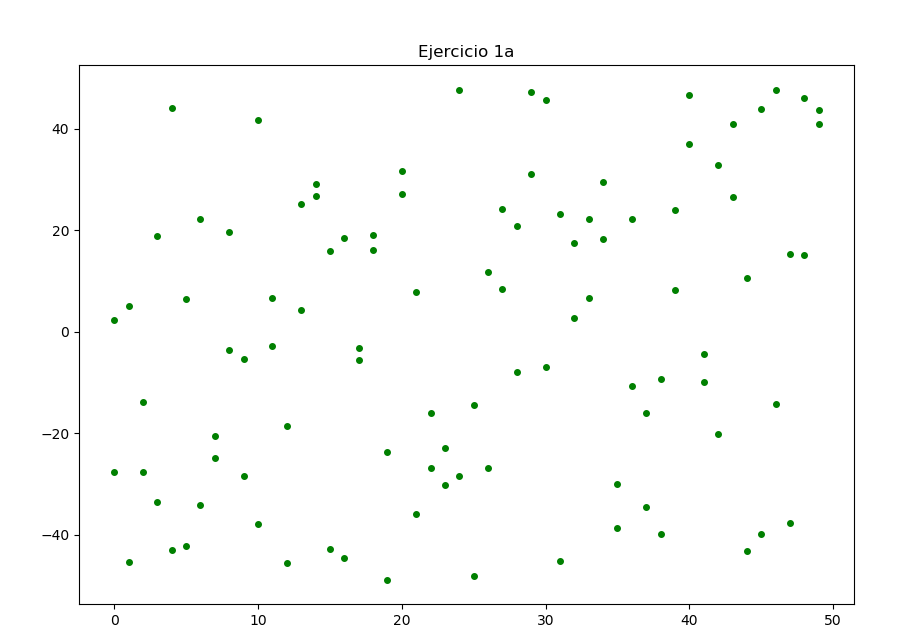
\includegraphics[width=0.7\linewidth]{screenshot001}
			\caption{}
			\label{fig:screenshot001}
		\end{figure}
		
		
		\item 
		\textbf{Considere N = 50, dim = 2, rango = [5,7] con simula\_gaus(N,dim,rango).}

		
		Esta grafica es la generada por simula\_gaus(N,dim,rango).
		
	\begin{figure}[H]
		\centering
		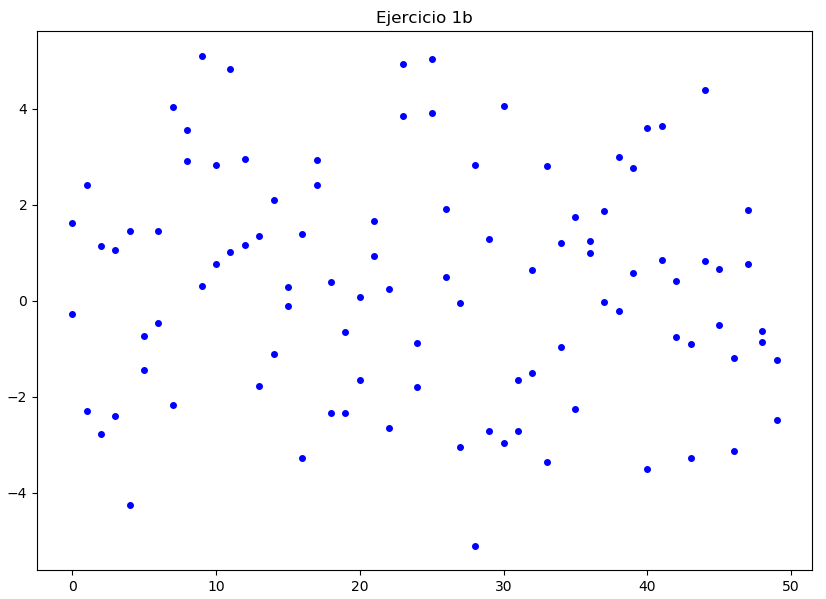
\includegraphics[width=0.7\linewidth]{screenshot002}
		\caption{}
		\label{fig:screenshot002}
	\end{figure}
	
		
		
		 
	\end{enumerate}
	\subsection{Ejercicio 2}
	\textbf{Con ayuda de la función simula\_unif() generar una muestra de puntos 2D a los que añadir una etiqueta usando el signo de la función f(x,y) = y -ax -b, es decir el signo de la distancia de cada punto a la recta simulada con simula\_recta()}
	
	\begin{enumerate}
		\item 
		\textbf{Dibujar de forma aleatoria los puntos muestren el resultado de su etiqueta, junto con la recta usada para ello. (Observe que todos los puntos están bien clasificados respecto la resta)}
		
		\begin{figure}[H]
			\centering
			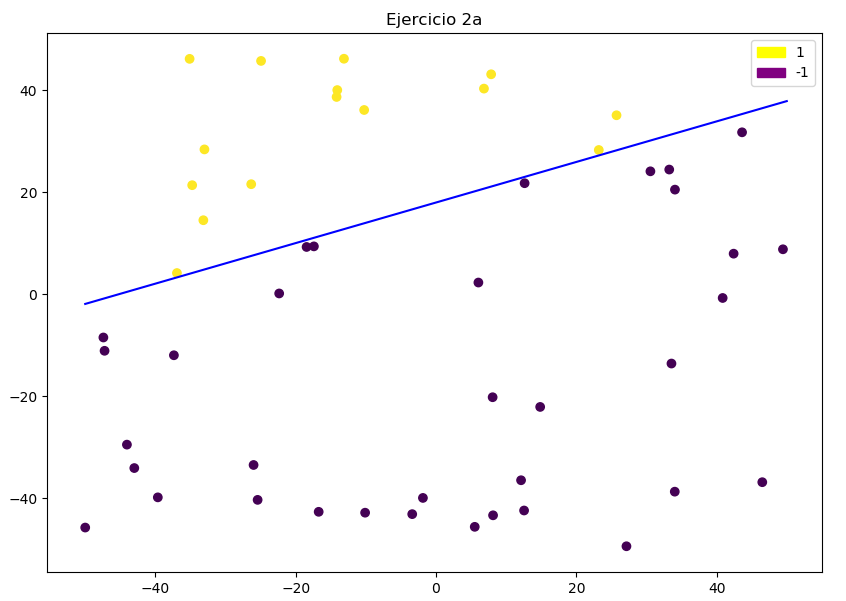
\includegraphics[width=0.7\linewidth]{screenshot003}
			\caption{}
			\label{fig:screenshot003}
		\end{figure}
		
		Como se ve en la grafica los putos amarillos son los que se encuentran por encima de la recta y los morados los inferiores. La recta separa perfectamente los puntos.
		
		\item 
		\textbf{Modifique de forma aleatoria un 10\% de las etiquetas positivas y otro 10\% de negativas y guarde los puntos con sus nuevas etiquetas. Dibuje de nuevo la grafica anterior. (Ahora hay puntos mal clasificados respecto la recta.)}
		
		\begin{figure}[H]
			\centering
			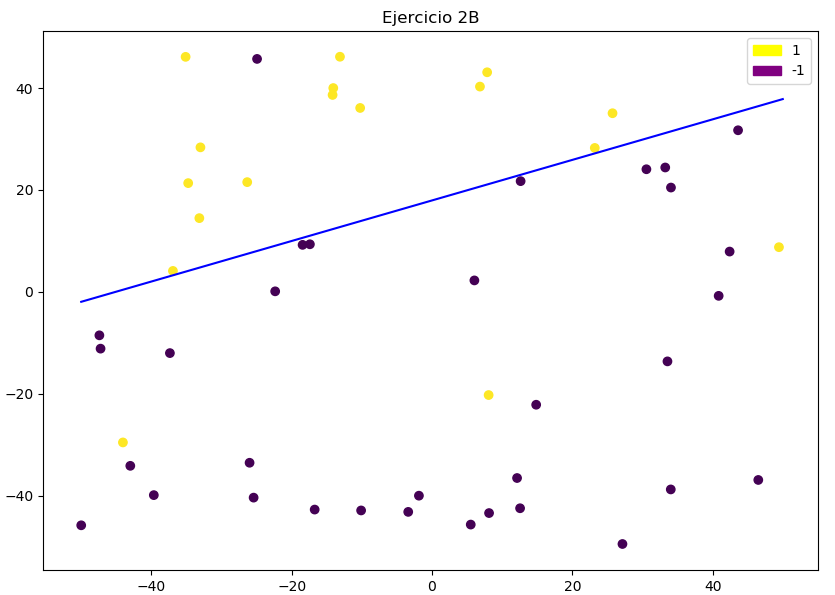
\includegraphics[width=0.7\linewidth]{screenshot004}
			\caption{}
			\label{fig:screenshot004}	 
		\end{figure}
		En este caso no se separan totalmente los puntos al cambiar algunos de signo. Estos puntos se ven claramente al tener el color contrario al que le pertenecería.
		
	\end{enumerate}

	\subsection{Ejercicio 3}
	\textbf{Supongamos ahora que las siguientes funciones definen la frontera de la clasificación de los puntos de la muestra en lugar de una recta.}
	
	\begin{enumerate}
		\item 
		\textbf{$f(x,y) = (x-10)^2 + (y-20)^2 - 400$}
		
		\item 
		\textbf{$f(x,y) = 0.5(x+10)^2 + (y-20)^2 - 400$}
		
		\item 
		\textbf{$f(x,y) = 0.5(x-10)^2 - (y+20)^2 - 400$}
		
		\item 
		\textbf{$f(x,y) = y-20x^2-5x+3$}
	\end{enumerate}

	\textbf{Visualizar el etiquetado generado en 2.2 junto con cada una de las gráficas de cada una de las funciones. Comparar las formas de las regiones y negativas de estas nuevas funciones con las obtenidas en el caso de la recta. ¿Son Estas funciones mas complejas mejores para clasificar que la función linea? ¿En que ganan a la función lineal? Explicar el razonamiento.}
	
	\begin{figure}[H]
		\centering
		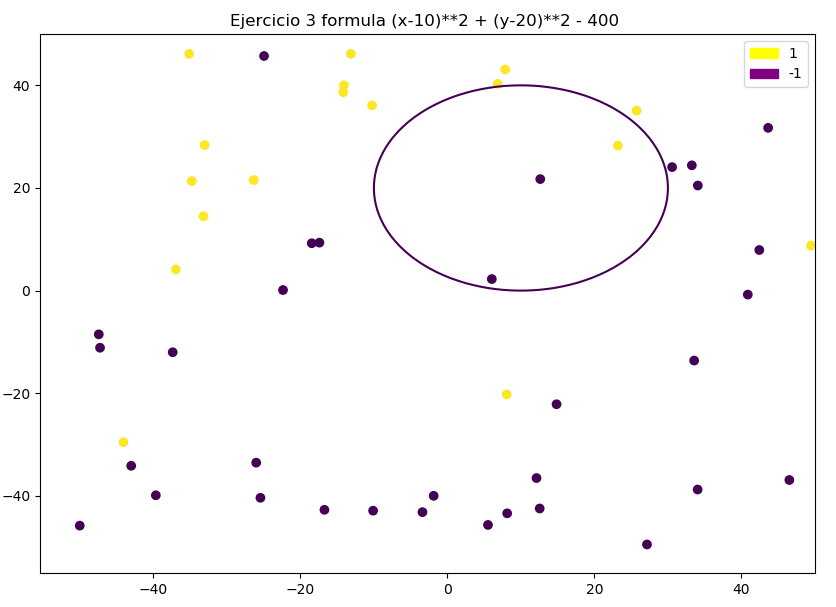
\includegraphics[width=0.7\linewidth]{screenshot005}
		\caption{}
		\label{fig:screenshot005}
	\end{figure}
	\begin{figure}[H]
		\centering
		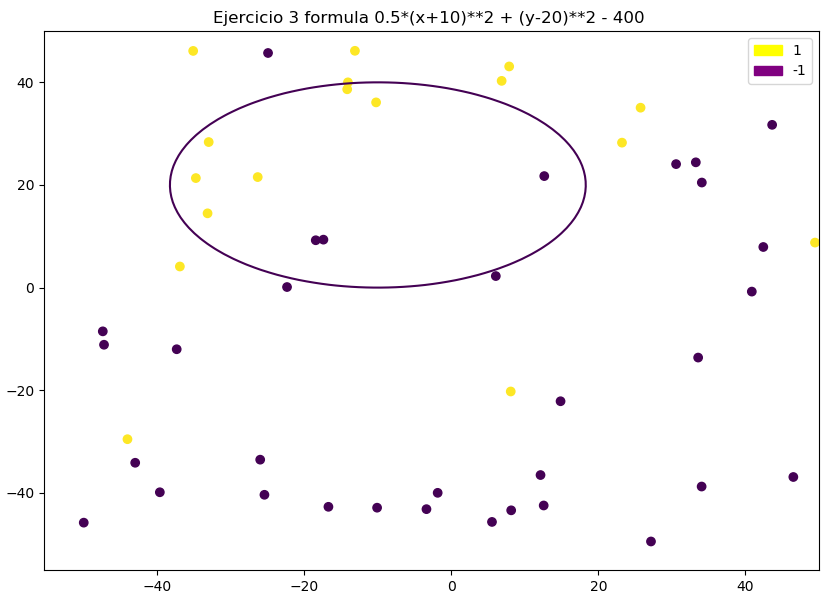
\includegraphics[width=0.7\linewidth]{screenshot007}
		\caption{}
		\label{fig:screenshot007}
	\end{figure}
	\begin{figure}[H]
		\centering
		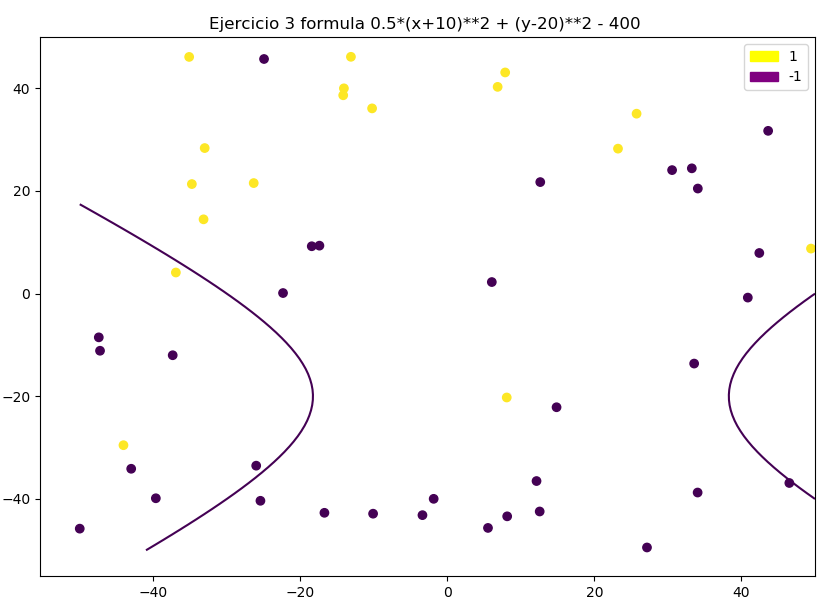
\includegraphics[width=0.7\linewidth]{screenshot008}
		\caption{}
		\label{fig:screenshot008}
	\end{figure}
	\begin{figure}[H]
		\centering
		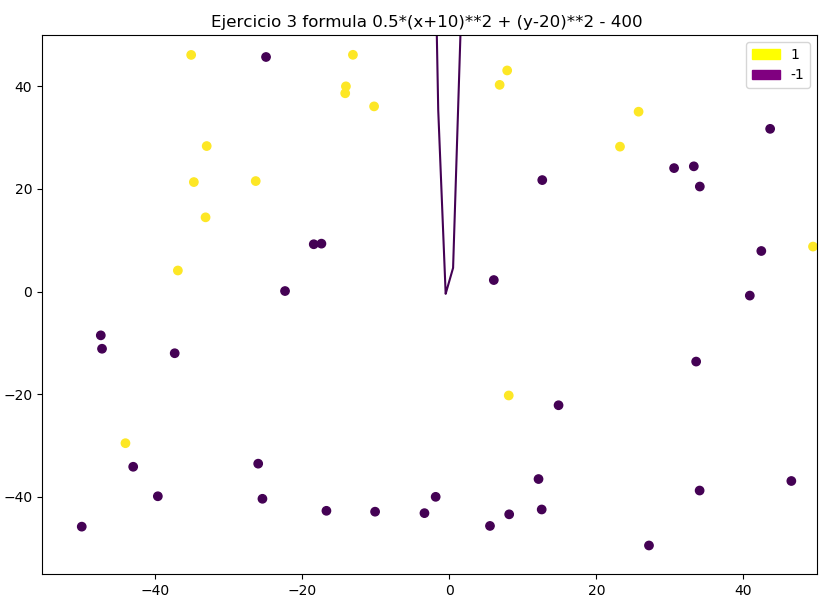
\includegraphics[width=0.7\linewidth]{screenshot009}
		\caption{}
		\label{fig:screenshot009}
	\end{figure}
	Si son mas complejas estas funciones pero 
	en este caso como los datos fueron generados para ser separados por un hiperplano estas formulas no se adaptan bien a los datos y los separan mucho peor que el hidroplano. 
	\newline
	
	Con estos datos las funciones propuestas en este ejercicio no mejoran en nada a el hiperplano. Esto nos demuestra que elegir funciones mas complicadas no tiene porque mejorar nuestro modelos. Se tiene que buscar el tipo de función que mas se adapte a nuestros datos.
	
	\newpage
	
	\section{Modelos Lineales}
	\subsection{Ejercicio 1}
	\textbf{Implementar la función ajusta\_PLA(datos,label,max\_iter,vini) que calcula el hiperplano solución de clasificación binaria usando el algoritmo PLA. La entrada datos es una matriz donde cada ítem con su etiqueta está representado por una fila de la matriz, label el vector de etiquetas ( cada etiqueta es un valor +1 o -1), max\_iter es el número máximo de iteraciones permitidas y vini el valor inicial del vector. La función devuelve los coeficientes del hiperplano}
	
	\begin{enumerate}
		\item 
		\textbf{Ejecutar el algoritmo PLA con los datos simulados en el apartado 2.1 de la seccion 1. Inicializar el algoritmo con: a) vector cero y b) con vectores de números aleatorios en [0,1] (10 veces). Anotar el número medio de iteraciones necesarias en ambos para converger. valorar el resultado relacionando el punto de inicio con el numero de iteraciones.}
		\newline
		
		Con estos datos el PLA puede separar los datos perfectamente al ser posible usar un hiperplano para esto.
		\begin{figure}[h]
			\centering
			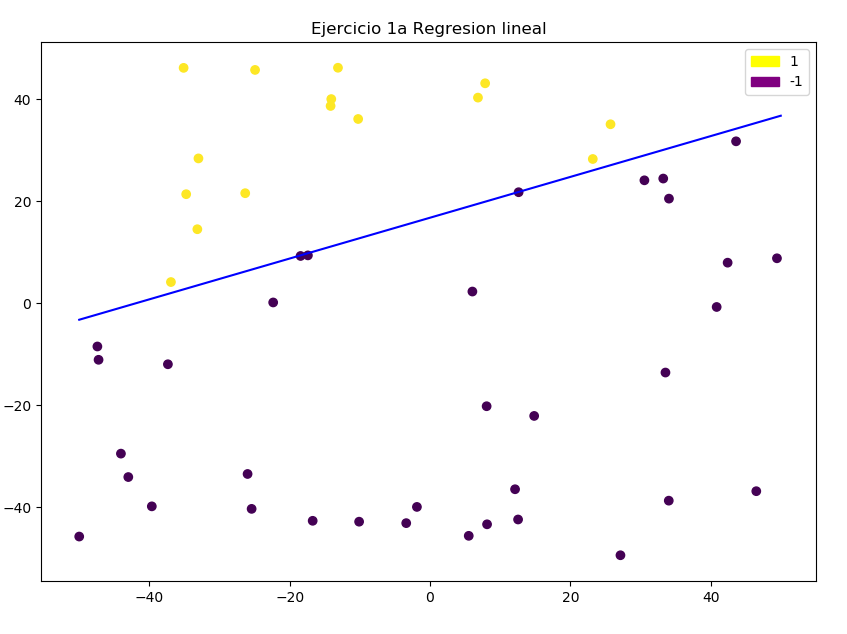
\includegraphics[width=0.7\linewidth]{screenshot010}
			\caption{}
			\label{fig:screenshot010}
		\end{figure}
		
		Cuando empezamos con el vector de 0 se alcanza en 86 iteraciones y con el vector aleatorio lo alcanzamos en 78.2 de media. Las dos opciones no alcanzan el máximo de iteraciones que en mi caso es 100. Con el vector elegido aleatoriamente nos da mejores resultados.
		
		
		\item 
		\textbf{Hacer lo mismo que antes usando ahora los datos del apartado 2.2 de la sección 1. ¿Observa algún comportamiento diferente? En caso afirmativo diga cual y las razones para que ello ocurra.}
		\newline
		
		En este caso como se le metió ruido y estos puntos cambiados de signo nos hacían los datos imposible de separar por un hiperplano y por esto no converge y siempre utiliza el máximo de iteraciones que le pasemos al algoritmo.
		
		\begin{figure}[H]
			\centering
			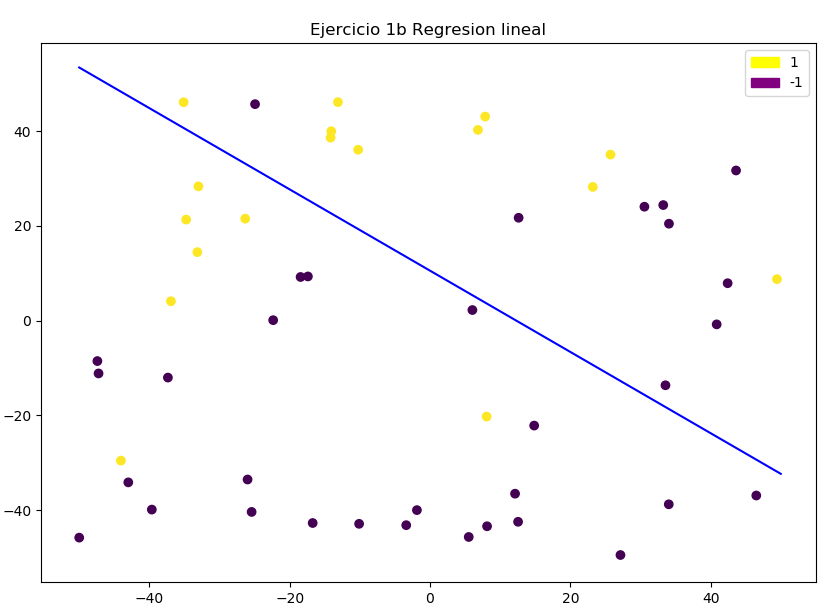
\includegraphics[width=0.7\linewidth]{screenshot011}
			\caption{}
			\label{fig:screenshot011}
		\end{figure}
	\end{enumerate}
		
		\subsection{Ejercicio 2}
		
		\textbf{En este ejercicio crearemos nuestra propia función objetivo f (una probabilidad en este caso) y nuestro conjunto de datos D para ver como función regresión logística. Suponemos por simplicidad que f es una probabilidad con valores 0/1 y por tanto la etiqueta y es una función determinista de x.}
		\textbf{Consideramos d = 2 para que los datos sean visualizables, y sea X = [0,2]x[0,2] con probabilidad uniforme de elegir cada $\mathbf{x} \in \mathcal{X}$. Elegir una línea en el plano que pase por X como la frontera entre f(x) = 1 (donde y toma valores +1 y f(x) = 0 (donde y toma valores-1), para ello seleccionar dos puntos aleatorios del plano y calcular la línea que pasa por ambos. Seleccionar N = 100 puntos aleatorios $\left\{\mathbf{x}_{n}\right\}$ de X y evaluar las respuestas $\left\{y_{n}\right\}$ de todos ellos respecto de la frontera elegida. }
		\newline
		
		Los datos los generaremos con las siguientes lineas.
		\newline
		Obtenemos la recta.
		\newline
		a,b = simula\_recta((0,2)).
		\newline
		Generamos los puntos y las etiquetas.
		\newline
		X=simula\_unif(100,2,(0,2))
		\newline
		Y = np.sign(X.T[1] - a * X.T[0] -b)
		
		
		\begin{enumerate}
			\item 
			\textbf{Implementar Regresión Logística con gradiente descendente estocástico bajo las siguientes condiciones:}
			\newline
			Para el algoritmo del gradiente descendente he utilizado el código de la practica anterior. He modificado la forma de obtener los pesos utilizando la formula de la regresión lineal.
			$\nabla_{{w}} E_{\mathrm{in}}(\mathbf{w})$ 
			$=\frac{1}{N} \sum_{i=0}^{N}-y_{i} \mathbf{x}_{i} \sigma\left(-y_{i} \mathbf{w}^{\mathrm{T}} \mathbf{x}_{i}\right)$
			donde $\sigma(x)=\frac{1}{1+e^{-x}}$
			
			
			\begin{enumerate}
				\item
				\textbf{Iniciar el vector de pesos con valores 0.}
				
				\item 
				\textbf{Para el algoritmo cuando $\left\|\mathbf{w}^{(\mathrm{t}-1)}-\mathbf{w}^{(\mathrm{t})}\right\|<0,01$ donde $\mathbf{W}^{(t)}$ denota el vector de pesos al final de la época t. Una época es un pase completo a través de los N datos.}
				
				\item
				\textbf{Aplicar una permutación aleatoria, $1,2, \ldots, N$ , en el orden de los datos antes de usarlos en cada época del algoritmo.  }
				
				\item 
				\textbf{Usar una tasa de aprendizaje de n = 0,01}
			\end{enumerate}
		El algoritmo nos da la siguiente grafica.
		\begin{figure}[H]
			\centering
			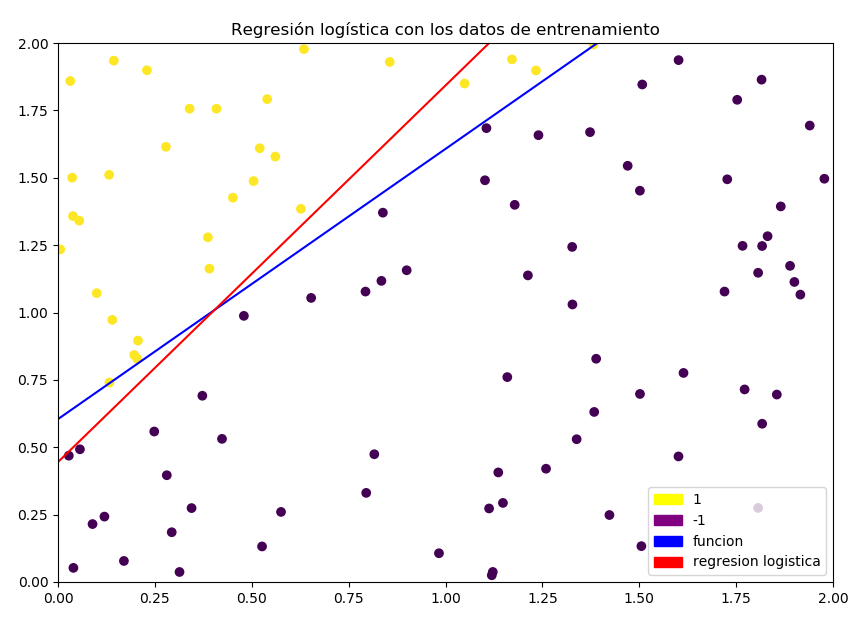
\includegraphics[width=0.7\linewidth]{screenshot013}
			\caption{}
			\label{fig:screenshot013}
		\end{figure}
		Como se ve no llega a ajustar del todo bien debido a que fijamos que parar cuando la resta de pesos de menos que 0.01. Para que se ajustara mejor se tendría que reducir ese valor y darle mas numero de iteraciones máximo.
		
		\item 
		\textbf{Usar la muestra de datos etiquetada para encontrar nuestra solución g y estimar $E_{{ out }}$ usando para ello un numero suficientemente grande de nuevas muestras $(>999)$}
		
		En mi caso he obtenido una muestra de 3000 puntos con las siguientes lineas.
		\newline
		
		x\_test=simula\_unif(3000,2,(0,2))
		\newline
		y\_test = np.sign(x\_test.T[1] - a * x\_test.T[0] -b)
		
		En la grafica muestro en azul la linea de la función utilizada para clasificar los puntos y la linea roja sera nuestra regresión logística.
		\begin{figure}[H]
			\centering
			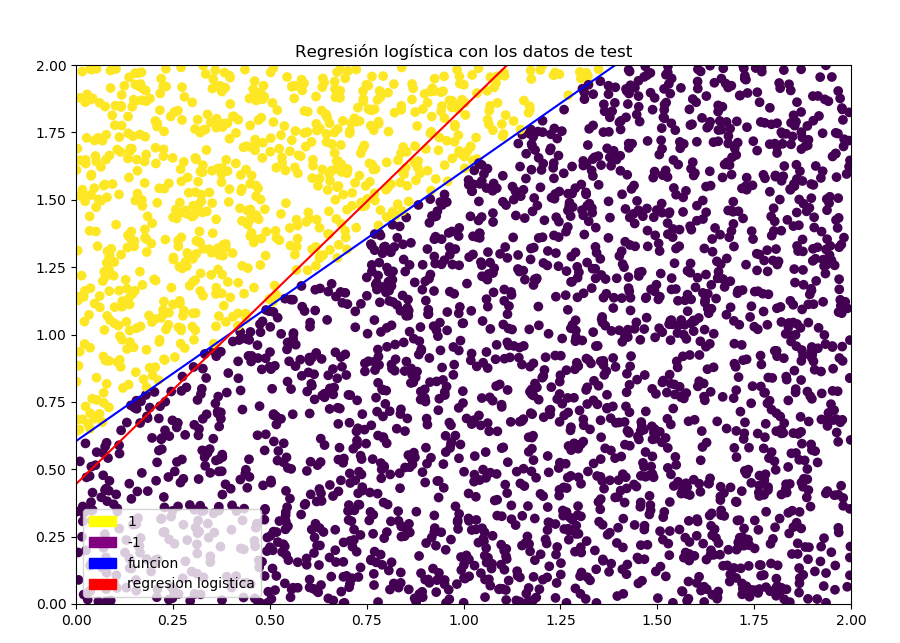
\includegraphics[width=0.7\linewidth]{screenshot012}
			\caption{}
			\label{fig:screenshot012}
		\end{figure}
		El error que nos da es de 0.0416
		
		\end{enumerate}
		
		\newpage
		
		\section{Bibliografía}
		
		Para dibujar las graficas del ejercicio 3 del primer apartado, he utilizado el código dado en la siguiente pagina:
		\newline
		https://stackoverflow.com/questions/32092899/plot-equation-showing-a-circle
	
	
	
	
	
	
	
 
  
\end{document}